\documentclass[11pt]{article}
\usepackage{amsmath}
\usepackage{amssymb}
\usepackage{cite}
\usepackage{microtype}
\usepackage[english]{babel}
\usepackage[labelsep=period, font=small]{caption}
\usepackage[margin=3.6cm]{geometry}
\usepackage{graphicx}
\usepackage[utf8]{inputenc}
\usepackage{listings}
\usepackage{mdframed}
\usepackage{float}
\usepackage{wisjab}
\usepackage{xcolor}
\usepackage{subfig}

\frenchspacing
\DisableLigatures[f]{}
\parindent=20pt

\definecolor{medgreen}{rgb}{0.0, 0.6, 0.0}
\definecolor{reddishmauve}{rgb}{0.6, 0.0, 0.3}
\lstset{language=Python, showstringspaces=false, numberfirstline=false, breaklines=true, numbers=left, stepnumber=1, tabsize=4,
basicstyle=\ttfamily, numberstyle=\tiny, commentstyle=\color{medgreen}\rmfamily, stringstyle=\color{reddishmauve}, keywordstyle=\color{blue}}

\DeclareMathOperator*{\argmin}{arg\,min}
\DeclareMathOperator*{\argmax}{arg\,max}
\def\tab{\hspace*{1cm}}

\def\urgent#1{{\LARGE\color{red}#1}}
\def\tvs{\textvisiblespace}

\author{Anonymous [s\,$*******$] and Unknown [s\,$*******$]}
\title{\textsc{\Huge neural networks}\\Assignment II\\[6mm]\large\bf Deep learning challenge}

\begin{document}
\maketitle
\section{Introduction}
Over the recent years, more and more people from all over the globe have taken a step into the digital world. However, not every one of them has access to a non-standard keyboard, or the willingness to use one. This can create confusion, especially among those whose native language contains characters that are variations of the standard Latin alphabet (which, in fact, comprises most of Europe). Therefore, the development of an algorithm which can aid such users in recognising substituted ASCII-type characters and replacing them by the correct variant, is necessary. In this research we apply a deep learning method to this problem, specifically for the Hungarian language.\par
The Hungarian alphabet consists of 44 graphemes, 9 of which contain diacritics. These are the vowels á, é, í, ó, ö, ő, ú, ü, ű and their uppercase versions. It is important to note that these are really different from the Latin a, e, i, o, u, and are considered distinct letters. As such, words which differ only by one such vowel -- and which would be written identically in ASCII format -- can have different meanings. Examples are: \textit{öt} (``five'') - \textit{őt} (``him''/``her'', accusative case); \textit{hat} (``six'') - \textit{hát} (``back''); \textit{kor} (``age'') - \textit{kór} (``disease'') - \textit{kör} (``circle'').\par
Our applied deep learning method is based on the technique of convolutional neural networks. These networks are known for their capability to detect patterns (also dubbed \textit{features}) in images, so as to determine what is depicted. In this sense, they mimic human visual recognition. Our objective is to investigate how well this type of networks is suited for pattern detection in written text, in order to choose correctly which diacritic should be placed on each encountered vowel.
\section{Approach}
If we want to attack the problem with a convolutional network, we somehow need to represent the information surrounding a vowel, which serves as context for picking the right letter variant, as some kind of image. Fortunately, since we are working with ASCII values as input, this is straightforward. For each vowel, we construct an $S$-vector (that is, a vector of length $S$) containing the values of the $S-1$ neighbouring characters (both left and right) and the vowel itself, which appears somewhere in the middle. In other words, we look at $R$ characters to the right of the vowel, $S-1-R$ characters to the right and the vowel itself. We chose to include spaces and punctuation characters in these vectors, as certain letters can occur more often at the beginning and end of words, and certain words may precede or follow punctuation marks more frequently. The output is represented as a one-hot 4-vector $\vc{v}^{(i)}$, $v^{(i)}_j=\delta^i_j$ for each of the five vowels, which indicates the right variant. Here, $\vc{v}^{(0)}$ stands for no diacritic (a, e, i, o, u), $\vc{v}^{(1)}$ represents an acute accent (á, é, í, ó, ú), $\vc{v}^{(2)}$ means a diaeresis (ö, ü) and $\vc{v}^{(3)}$ is used for a double acute accent (ő, ű). The vectors $\vc{v}^{(2)}$ and $\vc{v}^{(3)}$ applied to a, e, i return the no-diacritic and acute accent versions; however, these combinations do not occur in the input data.\par
By assuming that surrounding characters can serve as context information, we partly rely on the grammatical patterns Hungarian words exhibit. This is most apparent in the use of suffixes (which play the role of prepositions in English) that may change whether a vowel in the stem of a word bears a diacritic or not. For instance: the \textit{a} in \textit{órával} (``with the clock'') is written with an acute accent, while the \textit{a} in \textit{óra} (``clock'') is accentless. A convolutional network could be able to learn such suffixes as features, and possibly similar letter structures under which diacritics occur more frequently.\par
Since we are working from the viewpoint of character sequences, a recurrent network is not in our field of interest. There are several reasons for this. First of all, we want the network to look ahead in the text, so as to capture suffixes as well. Recurrent networks tend to take only the preceding information into account, which is not sufficient for our practices. Furthermore, we do not need a full-scale language model to describe our diacritics; after all, the text is already given, and the likelihood that a diacritic appears in a certain position based on previous characters may be better captured in features (convolutional kernels) than a list of probabilities. Furthermore, we do not want to build a generative algorithm.\par
The network is constructed as follows. We use two convolutional layers, each with their own linear rectifier (ReLU) activators:
\begin{align}
f_\text{act}(x)=\max(0, x).
\end{align}
The convolution runs over a zero-padded sequence, such that the resulting vectors are of the same size. The first layer learns $F/2$ features, where $F$ is a parameter that may be varied. After ReLU activation, these vectors are then pooled with a $2\times1$ pooling layer. This procedure is repeated to produce a $(S/4)\times F$ tensor of learning parameters. For this reason, $S$ should be a multiple of 4. Then, a fully connected layer of $N$ nodes is added, which ends in four output nodes. The predicted variant is then the argmax of these four values, in the same order as the aforementioned one-hot vectors. In order to reduce overfitting, we apply dropout to the fully connected layer. The topology of the network is shown in figure \ref{fig:convnet_topo}.\par
The vector-vector pairs were generated from several 20\textsuperscript{th} century literary works\cite{1, 2, 3, 4, 5}.
\begin{figure}[t]
\centering
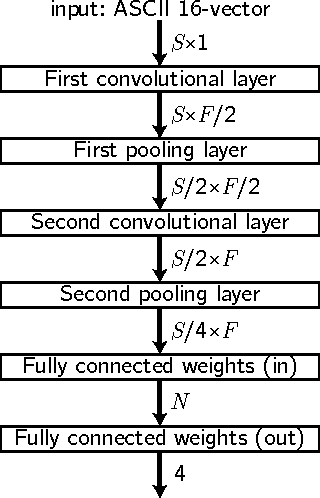
\includegraphics[scale=1]{convnet_topo.pdf}
\caption{The topology of the convolutional network used in our research. The input is a list of $S$-vectors, and the output is a one-hot 4-vector as described above. Dropout occurs between the last two stages.}
\label{fig:convnet_topo}
\end{figure}
\section{Evaluation methods}
We define an epoch as a sequence of 100 learning steps, where each of these steps take a random input-output pair from the training set. Initially, we choose $F=64$, $N=256$, $S=16$ and $R=8$. The size of the kernels is set to equal $S/2$. We run our experiments using multiple different parts of the data set, consisting of 100,000--150,000 training examples.\par
We also check the influence of the look width $S$ on the test set accuracy of the network, by training the network in 250,000 epochs for different values of $S$. The result of this measurement is shown in figure \ref{fig:variS}.
\section{Results and discussion}
\begin{figure}[!t]
\centering
\includegraphics[width=0.8\textwidth]{variS.pdf}
\caption{Test set accuracies for different look width values: $S\in\{8, 12, 16, 20\}$. We chose $R=S/2$, and left other parameters the same.}
\label{fig:variS}
\end{figure}
After training the convolutional network for 10,000 epochs with the initial parameters, we obtain an accuracy of 0.799 on the training set. In this case, the test set accuracy is 0.751. Although this may sound reasonable, it is in fact rather poor. After all, upon inspection of the training and test data, we discovered that approximately 72--75\% of the vowels is accentless. When we look at the actual output of the network at this stage (that is, applied to ASCII text), we see that no diacritics are placed at all. Apparently, the network learns not to change the ASCII text, since it thinks it is the most likely way to proceed correctly.\par
When we train the network longer, we can slowly see the accuracy rise. At 250,000 epochs, we obtain a training set accuracy of 0.913, and a test set accuracy of 0.800. This time, we observe diacritics actually appearing in the output text. Just over half of them -- 58.6\% to be precise -- are also in the correct position, although unnecessary diacritics still appear (that is, a character which is accentless in the correct Hungarian word receives is given a diacritic by the network). However, many needed diacritics are still missing, which accounts for most of the 0.200 accuracy that is still lacking.\par
What is striking is that short words, consisting of five characters at most, are often correctly recognised by the network. One possible explanation for this could be that only very few, if any, variations of these short words exist. This makes it easier for the network to perform well on these words. Furthermore, short sequences are easier to learn than long ones; for example, it should take the algorithm less effort to recognise \tvs\textit{ő}\tvs~(``he/she'') than \tvs\textit{végighömpölyödik}\tvs~(meaning something along the lines of ``all the way down''). This is augmented by the fact that short words tend to appear more often in text than long ones.\par
We have looked at the possibility of improving the performance on long words by allowing the network to look further than only 16 characters in total. This could provide more context for it to build the learning features upon, possibly enhancing their quality. A downside of this is that more context can mean more perceived randomness in the input. After all, character sequences in natural language can seem rather random if nothing about the etymology and grammatical structure of the words is known. As we can see in figure \ref{fig:variS}, the test set accuracy plummets to 0.75 when we choose $S=20$, suggesting that any increase beyond that value will yield nothing beneficial.\par
Another point of interest is the amount of noise that occurs in our data set. While scanning through the text, we found a number of Latin and German phrases intertwined with the Hungarian sentences. Although we did remove some of them, there is a possibility that a few still remained, acting as noise in the data.\par
It must be noted that we never fed the network any information about the words themselves beforehand, as we expected the detection of character patterns to be sufficient. It seems, however, that this severely hampers the process of learning where to properly place the diacritics, as character patterns turn out to be very complex and therefore hard to learn. This explains why Google translate is capable of picking the right spelling when only ASCII characters (or even wrong character variants, for that matter) are used. For instance, typing \textit{ora}, \textit{öra} or \textit{őra} will immediately turn up the translations for \textit{óra} (``clock''). The translator can simply look up words in a dictionary and choose the one that matches the query. However, this is not guaranteed to work well when context matters. Take a look at the following translations:\\[2mm]
\tab Hungarian: \textit{A naccságos tisztelendő úrral akarunk beszélni, hogy legalább az áldást\break\tab aggya ránk}\\
\tab Translation: ``We want to talk to a gentle, honorable gentleman, to at least bless\break\tab us''\\[2mm]
\tab Hungarian (without diacritics): \textit{A naccsagos tisztelendo urral akarunk beszelni,\break\tab hogy legalabb az aldast aggya rank}\\
\tab Translation: ``We want to talk to the vicious respectable leader that the aldast is\break\tab the lowest rank''\\[2mm]
We can see a big difference in the output of the translator. Apparently it is not always able to choose the right variant, leading to confusion and an incorrect translation. Naturally, this does not imply that dictionary-based methods are worthless; however they may not be able to tell the whole story.
\newpage
\section{Conclusion}
We explored a convolutional neural network, trained for pattern detection in written text. The network was specificallly trained to learn the diacritic placement in hungarian text. The network was able to obtain a training set accuracy of 0.913 and test set accuracy of 0.800. We assumed that the character patterns would be enough information for the network to learn from. But this does not seem to be the case ( merely a 0.8000 accuracy). A better way of handling this problem could be by using a word level recurrent neural network that has been fed a hungarian dictionary. This way the network can choose between the variants of a word based on what contex the word takes place. 


recurrent netwerk dat woordenboek uit het hoofd kent doet het waarschijnlijk beter
Met alleen ongecontroleerd leren komen we er niet; verder hulpmiddelen nodig
\vspace*{\fill}
\begin{thebibliography}{x}
\bibitem{1}Á. Tamási. (1932) Ábel a rengetegben. ISBN 9631538931.
\bibitem{2}F. Molnár. (1907) A Pál utcai fiúk. 	ISBN 9789631191714 (2012).
\bibitem{3}G. Gárdonyi. (1901) Egri csillagok.
\bibitem{4}S. Rideg. (1943) Indul a bakterház. ISBN 9631522512 (1982).
\bibitem{5}Z. Móricz. (1920) Légy jó mindhalálig. ISBN 9631120252 (1980).
\end{thebibliography}
\end{document}
